\documentclass[12pt]{article}

% --- Pacotes essenciais
\usepackage[utf8]{inputenc}
\usepackage[T1]{fontenc}
\usepackage[english]{babel}
\selectlanguage{english}
\usepackage{geometry}
\usepackage{setspace}
\usepackage{graphicx}
\usepackage{amsmath}
\usepackage{booktabs}
\usepackage{lmodern}
\usepackage{microtype}
\usepackage{fancyhdr}
\setlength{\headheight}{29pt}
\usepackage{titlesec}
\usepackage{ragged2e}
\usepackage{amssymb}
\usepackage{bbm}
\usepackage{csquotes}
\usepackage{float}
\usepackage[backend=biber,style=authoryear,doi=false,isbn=false,url=true]{biblatex}
\addbibresource{biblio.bib}
\graphicspath{{../output/figures/}}
\makeatletter
\def\input@path{{../output/tables/}}  % search path for \input
\makeatother

% % Usar "&" antes do último autor (em refs e citações)
% \DeclareDelimFormat{finalnamedelim}{%
%   \ifnumgreater{\value{liststop}}{2}{\finalandcomma\addspace\&\space}{\addspace\&\space}%
% }
% % (opcional) manter separador entre múltiplos autores como vírgula + espaço
% \DeclareDelimFormat{multinamedelim}{\addcomma\space}


\usepackage[dvipsnames]{xcolor} % nomes de cores prontos (RoyalBlue, MidnightBlue, etc.)
\usepackage[colorlinks=true,
            linkcolor=RoyalBlue,    % títulos/refs internas
            urlcolor=RoyalBlue,     % URLs
            filecolor=black,
            citecolor=RoyalBlue % cor das citações (\textcite, \parencite)
]{hyperref}

% Custom commands
\newcommand{\R}{\mathbb{R}}
\newcommand{\N}{\mathbb{N}}
\newcommand{\E}{\mathbb{E}}
\renewcommand{\P}{\mathbb{P}}
\DeclareMathOperator{\Cov}{Cov}
\DeclareMathOperator{\Var}{Var}
\DeclareMathOperator{\std}{std}
\DeclareMathOperator*{\argmax}{arg\,max}
\DeclareMathOperator*{\argmin}{arg\,min}

% --- Margens e espaçamento
\geometry{a4paper, margin=1in}
\onehalfspacing

% --- Metadados
\newcommand{\Institution}{Escola de Economia de São Paulo (EESP)}
\newcommand{\Course}{Master's Thesis}
\newcommand{\AuthorName}{Esthevão Marttioly}
\newcommand{\PaperYear}{2026}
\newcommand{\PaperType}{Advisor: Bernardo Guimarães}
\newcommand{\PaperTitle}{Conditional Cash Transfers as \\
                        Stabilization Tool: a HANK Approach}

% --- Cabeçalho SÓ na primeira página
\pagestyle{plain} % padrão para o resto
\fancyhf{}
\lhead{\begin{tabular}[t]{@{}l@{}}\textbf{\Institution}\\\textbf{\Course}\end{tabular}}
\rhead{\begin{tabular}[t]{@{}r@{}}\textbf{\AuthorName}\\\textbf{\PaperYear}\end{tabular}}
\renewcommand{\headrulewidth}{0pt}

% --- Blocos visuais

\newcommand{\TitleBlock}{%
  % UMA ÚNICA LINHA fina antes do título
  \noindent\rule{\textwidth}{0.4pt}\par
  \begin{center}\small\bfseries \PaperType\end{center}
  \begin{center}\Large\bfseries \PaperTitle\end{center}
  \vspace{0.4cm}
}

% --- Seções
\titleformat{\section}{\large\bfseries}{\thesection.}{0.5em}{}
\titlespacing*{\section}{0pt}{1.2em}{0.6em}

\begin{document}

\thispagestyle{fancy}

\TitleBlock

\hrule
\vspace{1.0em}

%---------------------------------------------------
%	INTRODUCTION
%---------------------------------------------------
% \section{Introduction and Motivation}

% Fiscal transfers have been an important public policy instrument in various governments.
% Among the main examples, we can cite: \textit{Bolsa Família} (Brazil),
% \textit{Asignación Universal por Hijo} (Argentina), \textit{Progresa/Oportunidades} (Mexico),
% and \textit{Universal Credit} (United Kingdom). Although each program has its specificities,
% they all share the same objective: income redistribution.

% Whether a fiscal policy is targeted or universal makes all the difference when the issue is
% social justice. In standard macroeconomic models, all individuals are equals, meaning that
% transfers affect everyone in the same way \parencite{blanchard2007real}.

% However, households differ dramatically in their income, wealth, employment status, and propensity to
% consume. Microdata show that individuals have different marginal propensities to consume (MPC) depending
% on their income and credit constraints \parencite{kaplan2014model}.

% Therefore, a heterogeneous agent model is crucial to understand the impacts and differences between
% targeted and universal fiscal policies. In Heterogeneous Agent New-Keynesian (HANK) models, these differences
% matter a lot: the same transfer budget produces very different aggregate and distributional outcomes
% depending on targeting \parencite{auclert2025fiscal,kaplan2014model}.

% Literature has studied the effects of police targeting primarily in relation to police funding: whether
% through debt or taxes \parencite{mckay2016role}. Some other articles have studied the presence of fiscal
% transfers and unemployment insurance, mostly in isolation \parencite{krueger2016distribution,bartal2024consumption}.

% The idea behind this project is to systematically compare the effects of different fiscal policies to
% a universal lump-sum transfer, in the presence of a negative shock to aggregate demand that triggers
% the transfers. To answer this, I aim to simulate different fiscal structures, such as transfers based
% on wealth, income, employment status, or hand-to-mouth status, in a structural HANK model with unemployment.


%---------------------------------------------------
%	MODEL
%---------------------------------------------------
\section{Model}

The setup is a standard New Keynesian model with incomplete markets and labor
supply risk. Time is discrete and runs from $t=0$ to infinity. There are four
types of agents in the economy: households, firms, labor unions, and the government.

Households are heterogeneous \parencite{aiyagari1994uninsured}, workers and
firms join in a formal-informal setup, and the rest of the economy follows
the textbook New Keynesian model \parencite{gali2015monetary}. There is no
aggregate uncertainty and the economy starts in the deterministic steady-state.

%---------------------------------------------------
%	HOUSEHOLDS
\subsubsection*{Households}
Assume there exists a continuum $i\in[0,1]$ of ex-ante identical households,
but experiencing idiosyncratic shocks in labor productivity and discount factor.

Households enjoy a CRRA-GHH utility over consumption $c_{i,t}$ and worked hours
$h_{i,t}$ \parencite{greenwood1988investment}\footnote{The GHH specification
assumes zero income effect, so that the hours decision is separable from the
consumption-savings problem.}, which we define
$u(\tilde c_{i,t}) =  u(c_{i,t} - v(h_{i,t}))$ as
\[
\max_{c_{i,t},h_{i,t}} \; \E_0\left[ \sum_{t=0}^\infty \beta^t
\frac{\tilde c_{i,t}^{1-\frac{1}{\gamma}}}{1 - \frac{1}{\gamma}}
\right],
\quad \text{with } v(h) = \psi \frac{h^{1+\frac{1}{\varphi}}}{1+\frac{1}{\varphi}}
\]
where $\gamma$ is the elasticity of intertemporal substitution
(EIS) and $\varphi$ is the Frisch elasticity of labor supply.

A household faces idiosyncratic labor productivity shocks $e_{i,t}$ with
$\E[e_{i,t}] = 1$, and discount factor heterogeneity
$\beta_i\in\{ \beta_L, \beta_H \}$, where there is $\omega_I$
impatient households. They can work in the formal or informal sector,
or be unemployed $s\in\{F,I,U\}$.Each sector has a specific productivity
$\theta^s_{i,t}$, re-drawn on each new offer.

Formal workers earn labor income
$(1-\tau_{\ell}) \theta_{i,t}^F w_t e_{i,t} h_{i,t}$,
where $w_t$ is the formal wage rate and $\tau_{\ell}$ is a fixed labor
income tax rate. While, informal workers receive benefits
$\theta_{i,t}^I w_t^I e_{i,t} h_{i,t}$,
where $w_t^I = \xi w_t$ and $\xi\in(0,1)$ is the wage gap.
Let $y_t(s,e)$ be this non-financial income,
\[
    y_t(s,e,\theta) = \begin{cases}
        (1-\tau_\ell) \theta^F w_t h_t e, &\text{if formal;} \\
        \theta^I w_t^I h_t e
            + T_t \cdot \mathbbm{1}[\text{eligible}],
            \quad &\text{if informal;} \\
        T_t, &\text{if unemployed}.
    \end{cases}
\]

We assume that formal wages are observable by the government, so that
only informal workers and unemployed may be eligible to receive
\textit{Bolsa Família} (BF). We assume that informal households are
eligible if $y_{i,t}(I,e,\theta) < \bar y$ and that the total benefit
size is $\text{BF}_t$.

Households save into liquid assets $a_{i,t}$ with ex-ante real
return $1+r_t = (1+i_{t-1})/(1+\pi_t)$, where $i_t$ represents the
nominal interest rate and $\pi_t$ denotes inflation.
They also receive lump-sum transfers $\tau_t$ by the government and dividends
$d_{i,t}$ from firms, which we assume to be proportional to productivity
$d_{i,t} = d_t \cdot e_{i,t}$\footnote{
    Dividends are proportional to productivity in order to
    increase inequality. We aim to perform robustness tests with other
    specifications.}.
Their budget constraint at time $t$ reads:
\[
c_{i,t} + a_{i,t} = (1+r_t) a_{i,t-1} + y_{i,t}(s,e) + d_{i,t} + \tau_t.
\]

Incomplete markets impose a borrowing constraint $a_{i,t} \geq \underline{a}$.
Frictions in the labor market imply formal households delegate their labor supply
decisions to labor unions, and thus take worked hours as given.
While, informal ones choose hours to maximize their utility, thus, for each $i$,
% this is novel, better to explain it later
\[
\psi \left( h \right)^{1/\varphi} = \theta  w^I e
\quad \Leftrightarrow \quad h^I(e)
= \left[ \frac{\theta w^I e}{\psi} \right]^\varphi.
\]

This generates a productivity cutoff for informal workers of
\[
\theta w^I e \left( \frac{\theta w^I e}{\psi}
\right)^\varphi < \bar y
\quad \Leftrightarrow \quad
e < e^* = \frac{\left( \psi^\varphi \bar y \right)^\frac{1}{1+\varphi}}{\theta w^I}.
\]

Such as \textcite{esteban2021labor} and \textcite{finamor2025labor},
given a sector $s$, we assume that each worker faces an exogenous
layoff probability $\delta_s$, and receives an offer from $s$ with
probability $\pi_s$. The worker accepts the offer with the higher
value, smoothed by additive idiosyncratic preference shocks explained later.

The Bellman Equation for each individual $i$ in sector $s\in\{F,I\}$ is
\begin{align*}
    V_t^s(a,e,\beta,\theta) = &\max_{\tilde c,a'} \Bigg\{
    \frac{\tilde c^{1-\frac{1}{\gamma}}}{1-\frac{1}{\gamma}}
    % - \psi \frac{h^{1+\frac{1}{\varphi}}}{1+\frac{1}{\varphi}}
    + \beta \E_t \!\bigg[ \delta_s V_{t+1}^U(.)
    + (1-\delta_s) \bigg( \\
    &\quad\qquad \pi_F (1-\pi_I) \max\!\left\{V_{t+1}^s(.,\theta), 
            V_{t+1}^F(.,\theta')\right\} \\
    &\quad\qquad + (1-\pi_F)\pi_I \max\!\left\{V_{t+1}^s(.,\theta), 
            V_{t+1}^I(.,\theta')\right\} \\
    &\quad\qquad + \pi_F \pi_I \max\!\left\{V_{t+1}^s(.,\theta), 
            V_{t+1}^I(.,\theta'), V_{t+1}^F(.,\theta')\right\} \\
    &\quad\qquad + (1-\pi_F)(1-\pi_I) V_{t+1}^s(.,\theta)
    \bigg) \bigg] \Bigg\} \\
    \text{s.t.} \qquad &c+a' = (1+r_t) a + y_t(s,e,\theta) + d_{i,t} + \tau_t \\
    &a' \in [\underline a, \infty), \qquad \tilde c = c - v(h),
\end{align*}
and for each unemployed worker is
\begin{align*}
    V_t^U(a,\beta) = &\max_{c,a'} \Bigg\{
    \frac{c^{1-\frac{1}{\gamma}}}{1-\frac{1}{\gamma}}
    + \beta \E_t \!\bigg[ (1-\pi_F)(1-\pi_I) V_{t+1}^U(.) \\
    &\quad\qquad + \pi_F (1-\pi_I) \max\!\left\{V_{t+1}^U(.),
            V_{t+1}^F(.)\right\} \\
    &\quad\qquad + (1-\pi_F)\pi_I \max\!\left\{V_{t+1}^U(.), 
            V_{t+1}^I(.)\right\} \\
    &\quad\qquad + \pi_F \pi_I \max\!\left\{V_{t+1}^U(.), 
            V_{t+1}^I(.), V_{t+1}^F(.)\right\}
    \bigg] \Bigg\} \\
    \text{s.t.} \qquad &c+a' = (1+r_t) a + y_t(U) + d_{i,t} + \tau_t \\
    &a' \in [\underline a, \infty).
\end{align*}

Formal workers maximize their utility taking hours as given,
so their labor disutility is internalized at the union level,
not by individual households. However, informal hours are chosen and
therefore included in the Euler Equation. Given their decision,
their consumption-equivalent income is
\[
w^I e h_t - v(h_t) = w^I e h_t -
\psi \frac{h_{i,t} h_{i,t}^{1/\varphi}}{1 + \frac{1}{\varphi}}
= \frac{w^I e h_t}{1+\varphi}.
\]

As in \textcite{caliendo2019trade}, before deciding, the households receive
an offer $A\in\{F,I,FI\}$ and draws a vector $\{\varepsilon^j\}$ over
the options $j\in\mathcal{S}$, with scale $\sigma_S$\footnote{
    $\sigma_S$ governs the smoothness of the decision. As $\sigma_S \to 0$
    it collapses to the deterministic $\max$.},
and picks the option $j$ maximizing $V^j + \varepsilon^j$.
This delivers a closed-form expected value,
\[
\P^{A}(j) = \frac{\exp\!\left( V^j/\sigma_S \right)}
{\sum_{k\in\mathcal{S}} \exp\!\left( V^k/\sigma_S \right)},
\qquad
\E\!\left[ \max_{j\in\mathcal{S}} \left\{ V^j + \varepsilon^j \right\} \right]
= \sigma_S \ln \sum_{j\in\mathcal{S}}
    \exp\!\left( V^j/\sigma_S \right)\footnote{
    We use a standard linear weighted approximation for the log-exp sum.
}.
\]

These shocks render the transition a differentiable function,
which allows it to be linearized when computing the sequence-space Jacobians,
as in \textcite{iskhakov2017endogenous}. Therefore, the sector transition
matrix $\Pi_t^s = \P(s'|s)$ is given by
\[
\Pi_t^s = \begin{bmatrix}
    (1-\delta_F) \phi_F(F) & (1-\delta_F) \phi_F(I) & \delta_F \\
    (1-\delta_I) \phi_I(F) & (1-\delta_I) \phi_I(I) & \delta_I \\
    \phi_U(F) & \phi_U(I) & \phi_U(U)
\end{bmatrix},
\]
where $\phi_s(s')$ is the probability of accepting an offer $s'$ given that
the worker is in sector $s$,
\begin{align*}
\phi_F(I) &= \pi_F \pi_I \, \P'^{FI}(I) + (1 - \pi_F) \pi_I \, \P^{I}(I),
\qquad \, \; \phi_F(F) = 1 - \phi_F(I), \\
\phi_I(F) &= \pi_F \pi_I \, \P^{FI}(F) + \pi_F (1 - \pi_I) \, \P^{F}(F),
\qquad \phi_I(I) = 1 - \phi_I(F), \\
\phi_U(F) &= \pi_F \pi_I \, \P^{FI}(F) + \pi_F (1 - \pi_I) \,\P^{F}(F), \\
\phi_U(I) &= \pi_F \pi_I \, \P^{FI}(I) + (1-\pi_F) \pi_I \, \P^{I}(I),
\qquad \phi_U(U) = 1 - \phi_U(F) - \phi_U(I).
\end{align*}

We denominate the steady-state size of each sector $s\in\{F,I,U\}$ as
$\alpha_s$, such that $\alpha_F+\alpha_I+\alpha_U=1$. Also, the size of
Bolsa Familia program is denominated by $\text{BF}$.

%---------------------------------------------------
%	FIRMS
\subsubsection*{Firms}
In the firm side, there is a representative final-good producer that aggregates
a continuum of $j\in[0,1]$ intermediate inputs produced by formal firms,
\[
Y_t = \left(
    \int_0^1 y_{j,t}^\frac{\varepsilon-1}{\varepsilon} \: dj 
\right)^\frac{\varepsilon}{\varepsilon-1},
\]
where $\varepsilon>0$ is a constant substitution elasticity (CES).

Each intermediate good $j$ is produced by a monopolistic competitive
firm $y_{j,t} = Z_{t} l_{j,t} $. They hire labor at real wage $w_t$ and set
a constant markup of $\mu = \frac{\varepsilon}{\varepsilon-1}$.
Hence, $P_t = \mu Z_t W_t$, and real wage equals $w_t = Z_t/\mu$ at every date
in steady-state. Firms' dividends are taxed at the same rate $\tau_{\ell}$ as
labor income, so $d_t = (1-\tau_{\ell}) (Y_t - w_t L_t)$, where
$L_t = \E[l_{j,t}]$ is the aggregate formal labor.

We assume sticky prices following \textcite{rotemberg1982monopolistic},
standard in Neo-Keynesian's literature. Such as \textcite{hagedorn2019fiscal},
the Phillips curve for price inflation is given by
\[
\ln(1+\pi_t) = \kappa \left[
\frac{w_t}{Z_t} - \frac{1}{\mu}
\right] + \frac{\ln(1+\pi_{t+1})}{1+r_{t+1}} \cdot \frac{Y_{t+1}}{Y_t},
\]

Additionally, there is a representative informal firm operating in a perfectly
competitive market and producing under constant returns to scale,
so $Y_t^I = w^I_t L_t^I$, where the steady-state wage gap $\xi = w_t^I / w_t$
is calibrated to match \textit{PNAD Contínua} data.

%---------------------------------------------------
%	UNIONS
\subsubsection*{Unions}
Nominal wages are assumed to be sticky as in \textcite{erceg2000optimal},
where unions set nominal wages to maximize agent utility subject to
\textcite{rotemberg1982monopolistic}'s adjustment costs.
We assume that unions allocate all formal labor hours uniformly across agents,
so $ h_{i,t} = h_t $ \parencite{auclert2025fiscal}.

Also, as in \textcite{hagedorn2019fiscal}, union's objective is to maximize
the utility of an agent with average consumption $\bar C_t = \int_0^1 c_{it}
\: di$, discounted by the average discount factor
$\bar \beta = \lambda_I \beta_L + (1-\lambda_I) \beta_H$
\parencite{auclert2021exchange}. This results in a Phillips curve for wage
inflation $\pi_t^w = (1+\pi_t) w_t / w_{t-1} $ given by
\[
\ln (1+\pi_t^w)
= \kappa_w \left[ \psi \cdot h_t^{1/\varphi} \cdot \tilde C_t^{1/\gamma}
- \frac{(1-\tau_\ell) w_t L_t}{\mu_w}  \right]
+ \bar \beta \ln (1+\pi_{t+1}^w).
\]

The Phillips Curve calculations for price and wage are found in the Appendix.

%---------------------------------------------------
%	GOVERNMENT
\subsubsection*{Government}
Monetary Policy follows a standard lagged Taylor Rule, without microfoundations
and only with an inflation target, $i_t = r^*_{t-1} + \phi \pi_{t-1} $,
where $r^*$ is the neutral real interest rate, and $\phi > 1$
\parencite{taylor1993follow}.

In the governmental sphere, we have a government that collects taxes, makes
transfers, and incurs debt; therefore, the government's budget constraint
is characterized by
\[
\tau_t + T_t \cdot \text{BF}_t + (1+r_t) B_{t-1} = B_t + \tau_\ell Y_t.
\]

We consider two types of government policy, a revenue-neutral and a deficit-financed.
The policymaker chooses a path of the conditional transfers and adjusts transfers
or debt such that the budget is balanced at each period.

The revenue-neutral policy sets a path of $T_t$ and adjusts transfers such that
\[
\tau_t = \tau_\ell Y_t - T_t \cdot \text{BF}_t - r_t \bar B,
\]
which means that the fiscal policy is passive and the monetary policy is active.
The nominal interest rate adjust at least one-for-one to changes in inflation.

However, governments normally finance themselves by increasing deficit and
issuing new debt. The deficit-financed policy sets a path of $T_t$ and adjusts
debt, keeping the nominal interest rate fixed $i_t = \bar i$.

This situation leads to larger multipliers and great inequality
\parencite{auclert2023trickling}. In the presence of nominal rigidity and non-
Ricardian consumer behavior, \textcite{angeletos2024can} show that fiscal
deficits of this sort self finance, so $\lim_{t\to\infty} B_t = \bar B$.

%---------------------------------------------------
%	MKT CLEARING
\subsubsection*{Market Clearing}
Finally, the asset, labor, and goods markets reach equilibrium
(Market Clearing Conditions). We define $\Lambda_t(s,\beta,e,a)$ as the household
distribution over a given period of time. First, the asset market reaches
equilibrium when household savings equal government bonds
\[
A_t = \int a_{i,t} \; d\Lambda_t(s,\beta,e,a) = B_t;
\]
the labor market clears when the share of employment in the workforce equals
the firm's demand for labor
\begin{align*}
    &L_t = \int \mathbbm{1}\{s_{i,t}=F \} \cdot \theta^F_{i,t} \cdot
            e_{i,t} \cdot h_{i,t} \; d\Lambda_t(s,\beta,e,a); \\
    &L_t^I = \int \mathbbm{1}\{s_{i,t}=I \} \cdot \theta^I_{i,t} \cdot
            e_{i,t} \cdot h_{i,t} \; d\Lambda_t(s,\beta,e,a);
\end{align*}
and the goods market clear when $Y + Y^I = C$. We set the goods market to clear
by Walras' Law. Lastly, the BF benefit is given to all eligible households,
\[
\text{BF}_t = U_t + \int \mathbbm{1}\{s_{i,t} = I, e_{i,t} < e^*\}
        \; d\Lambda(s,\beta,e,a).
\]

%---------------------------------------------------
%	DATA AND DESCRIPTIVE STATISTICS
%---------------------------------------------------
\section{Calibration}
\subsection*{Data}

To calibrate this model, we use Brazilian data and standard parameters
in HANK Literature. Most of the data refers to their average values in 2025.

The labor market moments were obtained in
\textit{Pesquisa Nacional por Amostra de Domicílio Contínua} (PNAD-C),
an annual survey reporting formality status, wages, weekly worked hours, etc.
This panel is interesting to match mainly the sector sizes and the worked hours,
for both formal and informal households. However, since it is a survey,
it might have under-reporting of informal firms.

Some general macroeconomic measures were also used, such as the Government Debt
(in the Brazilian National Treasure), the interest rates, and the inflation,
available in the \textit{Índice Brasileiro de Geografia e Estatística} (IBGE).
The Gini coefficient of wealth was obtained from the 2025 Global Wealth Report,
from UBS. \textit{Bolsa Família} data is available in \textit{Cadastro Único}
(CadÚnico), a platform with several statistics about the benefit.

In the future, we aim to gather information also in the
\textit{Relação Anual de Informações Sociais} (RAIS), a mandatory annual reporting
of firms, but without informality information and only up to 2003, and
\textit{Economia Informal Urbana} (ECINF), a survey conducted by IBGE that focus
on small business, specially informal ones.

%---------------------------------------------------
%	METHODS
%---------------------------------------------------
\subsection*{Methods}

The main computational methods are the Sequence-Space Jacobian (SSJ)
\parencite{auclert2021using}, and the Endogenous Grid Method (EGM)
\parencite{carroll2006method}. The EGM was combined with the discrete choice
among sectors using \textcite{iskhakov2017endogenous}.

The central idea of SSJ is to summarize the entire model by a matrix equation
$\mathbf{F}_t(\textbf{X},\textbf{Z}) = \textbf{0}$, where $\textbf{X}$ are the
endogenous variables and $\textbf{Z}$ are the exogenous ones. The Implicit
Function Theorem allows us to differentiate this system and obtain General
Equilibrium Jacobians, written as
\[
d\textbf{X} = \textbf{G} \, d\textbf{Z}
= -\textbf{F}_\textbf{X}^{-1} \textbf{F}_\textbf{Z} \, d\textbf{Z}.
\]

For each shock in \textit{Bolsa Família}, we can compute the Jacobian
$dC = \textbf{G}_{C,T} \, dT$ of the change in the conditional transfer
on household consumption. The Jacobian is computed by perturbing the
exogenous variable $T$ and solving the model for the new equilibrium,
then calculating the change in consumption $C$.

Further, we can compute the consumption response to a monetary shock
$dC = \textbf{G}_{C,i} \, di$ in the presence of the transfer, and compare
it to the counterfactual. We measure the stabilization effect of the transfer
as the difference between the response in the economy with the program and
in the $T=0$ counterfactual,
\[
\text{Stab}(T) = dC \, \big|_{T>0} - dC \, \big|_{T=0},
\]
read either as an impulse response or as the induced change in the volatility of
consumption $\Delta \!\Var(C_t)$, a program that smooths fluctuations delivers
$\Delta \!\Var(C_t) < 0$. This effect can be decomposed in a insurance and
a composition channel,
\[
d\textbf{X} = d\textbf{X}^\text{ins}
+ \left( d\textbf{X} - d\textbf{X}^\text{ins} \right)
= \textbf{G}^\text{ins} \, d\textbf{Z}
+ \left( \textbf{G} - \textbf{G}^\text{ins} \right) d\textbf{Z}.
\]

The sectoral block of the transition matrix $\Pi_t$ is endogenous and depends on
the continuation values, $\Pi_t = \Pi(\textbf{V}_t, \Lambda_t)$, where
$\textbf{V}_t = (V_t^F, V_t^I, V_t^U)$. The household's distribution evolves by
combining the asset policy with the Markov transition over the states,
$\Lambda_{t+1} = \mathcal{T} \!\left( \Pi_t, a_t(s,\theta,\beta,e) \right)$.
To solve the steady-state distribution, we iterate until $\Pi_t$ converges
to its fixed point, analogue to \textcite{aguirregabiria2007sequential}.

The insurance channel is captured by the frozen-$\Pi$. Holding sectoral sorting
fixed, the transfer relaxes the budget of unemployed and low-income informal
households, and, since these are high-MPC, it dampens the aggregate
response \parencite{auclert2024intertemporal}.

The composition channel is captured by the moving-$\Pi$ Jacobian, because the CCT
raises the value of informality relative to formal work, so workers are tilted
toward the informal sector, which is riskier. The insurance term is stabilizing,
while the composition is potentially destabilizing. The sign and magnitude of the
net effect are the quantitative answer to our question.

Letting the transition respond, $d\Pi_t = \Pi_{\textbf{V}} \, d\textbf{V}_t$,
yields the general equilibrium Jacobian $\textbf{G}$. This dynamic is
obtained as the dynamic analogue of the steady-state: given a shock path, we
iterate so that households' sectoral choices are consistent with the values
those very choices generate along the transition \parencite{auclert2021using}.

%---------------------------------------------------
%	CALIBRATION
%---------------------------------------------------
\subsection*{Calibration}

%---------------------------------------------------
\begin{table}[htbp]
\centering
\caption{External Calibration}
\label{tab:ext_calibration}
\small
\begin{tabular}{llcl}
\toprule
& \textbf{Description} & \textbf{Value} & \textbf{Source} \\
\midrule
\multicolumn{4}{l}{\textit{Households and Labor Market}} \\[2pt]
$\gamma$ & EIS & $\mEis$ & Standard in Literature \\
$\varphi$ & Informal Frisch Elasticity & $\mVarphi$ & Standard in Literature \\
$\psi$ & Disutility of Labor & $\mPsi$ & Normalization, $h_F = \mHF$ \\
$\beta_H$ & Patient's Discount Factor & $\mBetaHigh$ & $A/Y = B/Y = \mDatBGdp$ \\
$\delta_F$ & Job-Loss Probability to Formal & $\mDeltaF$ & PNAD-C Data \parencite{osorio2022montagem} \\
$\delta_I$ & Job-Loss Probability to Informal & $\mDeltaI$ & PNAD-C Data \parencite{osorio2022montagem} \\
[6pt]

\multicolumn{4}{l}{\textit{Firms}} \\[2pt]
$w$ & Average Wage & $\mW$ & Normalization, Reference \\
$\mu, \mu_w$ & Price Markup & $\mMu$ & \textcite{basu1997returns} \\
$\kappa$ & Price-NKPC Slope & $\mKappa$ & \textcite{hazell2022national} \\
$\kappa_w$ & Wage-NKPC slope & $\mKappaW$ & Equal to $\kappa$ \\
[6pt]

\multicolumn{4}{l}{\textit{Government and Monetary Policy}} \\[2pt]
$r^*$ & Neutral Real Interest Rate & $\mRstar$ & $4\%$ annual average \\
$\tau_\ell$ & Labor Income Tax Rate & $\mTauL$ & Average Tax Payroll \\
$\phi$ & Taylor Rule Coefficient & $\mPhi$ & Standard \parencite{taylor1993follow} \\
$B/Y$ & Government Debt-to-GDP Ratio & $\mDatBGdp$ & Brazilian National Treasure\\
$\phi_B$ & Sensitivity to Pay the Debt & $\mPhiB$ & $B$ converges within 10 years \\
[6pt]

\multicolumn{4}{l}{\textit{Bolsa Família}} \\[2pt]
$BF \cdot T / W$ & Bolsa Família Spending (\%Wage Bill) & $\mDatBFW$ & CadÚnico, PNAD-C \\
$\phi_F, \phi_I$ & Take-up at Zero Earnings & $\mDatPhiF, \mDatPhiI$ & PNAD-C \\
$\bar y_F, \bar y_I$ & Half-Coverage Threshold & $\mYbarF, \mYbarI$ & PNAD-C \\
$\sigma_F, \sigma_I$ & Smoothness of Eligibility & $\mDatSigF, \mDatSigI$ & PNAD-C \\
\bottomrule
\end{tabular}
\end{table}
%---------------------------------------------------
%---------------------------------------------------
\begin{table}[htbp]
\centering
\caption{Endogenous Calibration}
\label{tab:int_calibration}
\footnotesize
\begin{tabular}{llccccl}
\toprule
& \textbf{Description} & \textbf{Value} & \textbf{Target} & \textbf{Model} & \textbf{Data} & \textbf{Source} \\
\midrule
\multicolumn{4}{l}{\textit{Households}} \\[2pt]
$\beta_L$ & Impatient's Discount Factor & $\mBetaLow$ & Top 10\% & $\mModTopOneZero$ & $\mDatTopOneZero$ & WID World \\
$\omega_I$ & Share of Impatient Agents & $\mOmegaI$ & HtM Share & $\mModHtm$ & $\mDatHtm$ & Standard \\
$\sigma_S$ & Smoothness of Tastes & $\mSig$ & $\Delta_{IF}$ & $\mModDwIF$ & $\mDatDwIF$ & PNAD-C \\
[6pt]

\multicolumn{4}{l}{\textit{Labor Market}} \\[2pt]
$\pi_F, \pi_F^U$ & Formal Offer Probability & $\mPiF, \mPiUF$ & $F$ & $\mF$ & $\mDatF$ & PNAD-C \\
$\pi_I, \pi_I^U$ & Informal Offer Probability & $\mPiI, \mPiUI$ & $I$ & $\mI$ & $\mDatI$ & PNAD-C \\
$\rho_e$ & Persistence of Productivity & $\mRhoE$ & $\rho_1^y$ & $\mModAcOne$ & $\mDatAcOne$ & PNAD-C \\
$\sigma_e$ & Productivity Std. Dev. & $\mSdE$ & $q_{90}$ & $\mModQNineZeroF$ & $\mDatQNineZeroF$ & PNAD-C \\
$\mu_I$ & Informal Average Productivity & $\mMuI$ & $q_{50}^I$ & $\mModQFiveZeroI$ & $\mDatQFiveZeroI$ & PNAD-C \\
$\sigma_F$ & Formal Std. Dev. Produc. & $\mSigmaF$ & $q_{50}^F$ & $\mModQFiveZeroF$ & $\mDatQFiveZeroF$ & PNAD-C \\
$\sigma_I$ & Informal Std. Dev. Produc. & $\mSigmaI$ & $q_{75}^I$ & $\mModQSevenFiveI$ & $\mDatQSevenFiveI$ & PNAD-C \\
\bottomrule
\end{tabular}
\end{table}
%---------------------------------------------------

Each model period stands for one quarter and the computational time horizon is
100 quarters (or 25 years). We solve the steady-state equilibrium computationally
by Brent's method, internally calibrating parameters to clear the asset market,
the labor market, the government budget constraint, and the Phillips curves.
The external calibration is shown in table \ref{tab:ext_calibration} and
the endogenous calibration is in \ref{tab:int_calibration}.
The goods market was left untargeted to verify the Walras' Law.

The idiosyncratic productivity follows a log-normal $AR(1)$ process,
$\ln e' = \rho_e \ln e + \varepsilon^e$, with $\varepsilon^e \sim N(0,\sigma^2_e)$.
This is approximated by a finite Markov chain with $N_e$ grid points
\parencite{rouwenhorst1995asset}. We also assume a log-spaced grid for assets
and a log-normal sector productivity grid $\ln \theta^s \sim N(\mu_s, \sigma_s^2)$,
that is discretized by a Gauss-Hermite quadrature with $N_\theta$ nodes
\parencite{meghir2015wages}.

Each household has a $q = 0.10$ probability of drawing a discount factor
$(\beta_L, \beta_H)$, corresponding to an average type duration of 25 years,
used to capture a generation \parencite{auclert2025fiscal}.
This aims to capture similar results in relation to a life-cycle
overlapping generations with permanent ability shock model.
% pq delta_beta = 0.12 e w_I = 0.5   =>   Calibrar internamente!!

In the household preferences, elasticity of intertemporal substitution is standard
in literature $\gamma=0.5$\footnote{
    EIS $\gamma=0.5$ is consistent with micro estimates surveyed by
    \textcite{valickova2015financial}.}.
% The disutility of labor $\psi = 0.30$ is internally calibrated to normalize
% formal hours $h_F = 1.0$. At last, $\varphi = 0.15$ is chosen to approximate
% informal worked hours to PNAD-C Data, in average (model = $0.891$, data = $0.867$)
% and in standard error (model = $0.35$, data = $0.34$)\footnote{
%     We used the average of half the sample because, in the future,
%     high-productivity informal workers will choose for formalization.}.

% The labor market transition probabilities are defined to match the sector sizes
% in PNAD-C, $F = 50.5\%$ (data = $50.0\%$), $I = 44.0\%$ (data = $44.2\%$),
% and $U = 5.0\%$ (data = $5.8\%$). Their values are $p_{fi} = 0.11$, $p_{if} = 0.12$,
% $p_{ui} = 0.11$, $p_{uf} = 0.05$, and $p_{iu} = 0.02$. In the future, I am
% interested in estimating the sectoral transition risk in the PNAD-C, if feasible.

% escrever mu_F, mu_I, sigma_F, sigma_I    ->    dados PNAD
The output is normalized $Y=1.0$ and we defined $\mu = 1.11$, which is standard in
the HANK literature \parencite{kaplan2018monetary,auclert2025fiscal}\footnote{
    Markup $\mu=1.11$ is also consistent with the estimates of
    \textcite{basu1997returns}.}, and $\kappa = \kappa_w = 0.025$,
consistent with \textcite{hazell2022national} estimates.

Taylor Rule is pretty standard, with $\phi=1.5$ and $r^* = 1\%$, consistent with
a $4\%$ annual real interest rate for Brazilian economy \parencite{dos2024natural}.
The Government debt is set to $80\%$ of yearly GDP, consistent with Brazilian
National Treasure data. Wage tax is an average of all contributions levied on
the payroll, $\tau_\ell = 0.27$.   % ver esse tau_l

The \textit{Bolsa Família} statistics were obtained from the Cadastro Único\footnote{
    Available in \href{https://aplicacoes.cidadania.gov.br/vis/data3/data-explorer.php}{VIS DATA 3}
    and \href{https://paineis.mds.gov.br/public/extensions/observatorio-do-cadastro-unico/index.html}{Cadastro Único}.},
where we calibrated the $T/w$ ratio in steady-state to be equal to the data
from the Brazilian economy, with $T =$ R\$ 600 and $w =$ R\$ 4,294.
We also calibrated the \textit{Bolsa Família} threshold $\bar y$ to
match the actual size of the program\footnote{
    We used the average household size in PNAD-C to calculate a percentage
    estimate of the program.}.

%---------------------------------------------------
%	RESULTS
%---------------------------------------------------
\newpage
\section{Results}


\begin{figure}[H]
    \centering
    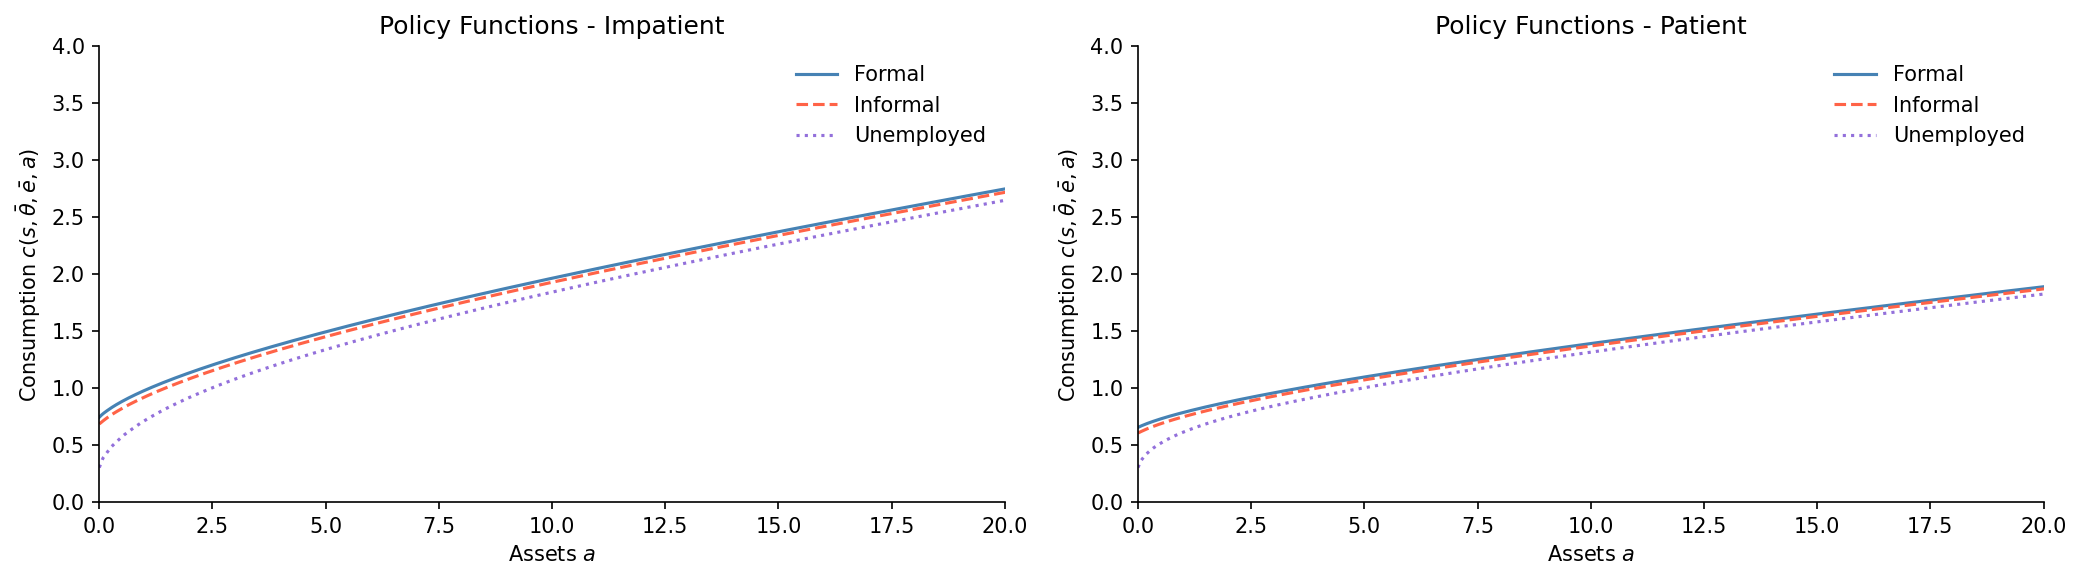
\includegraphics[width=1\linewidth]{consump_policy.png}
    \caption{Steady-State Consumption Policy Function}
    \label{fig:consump_policy}
\end{figure}


\begin{figure}[H]
    \centering
    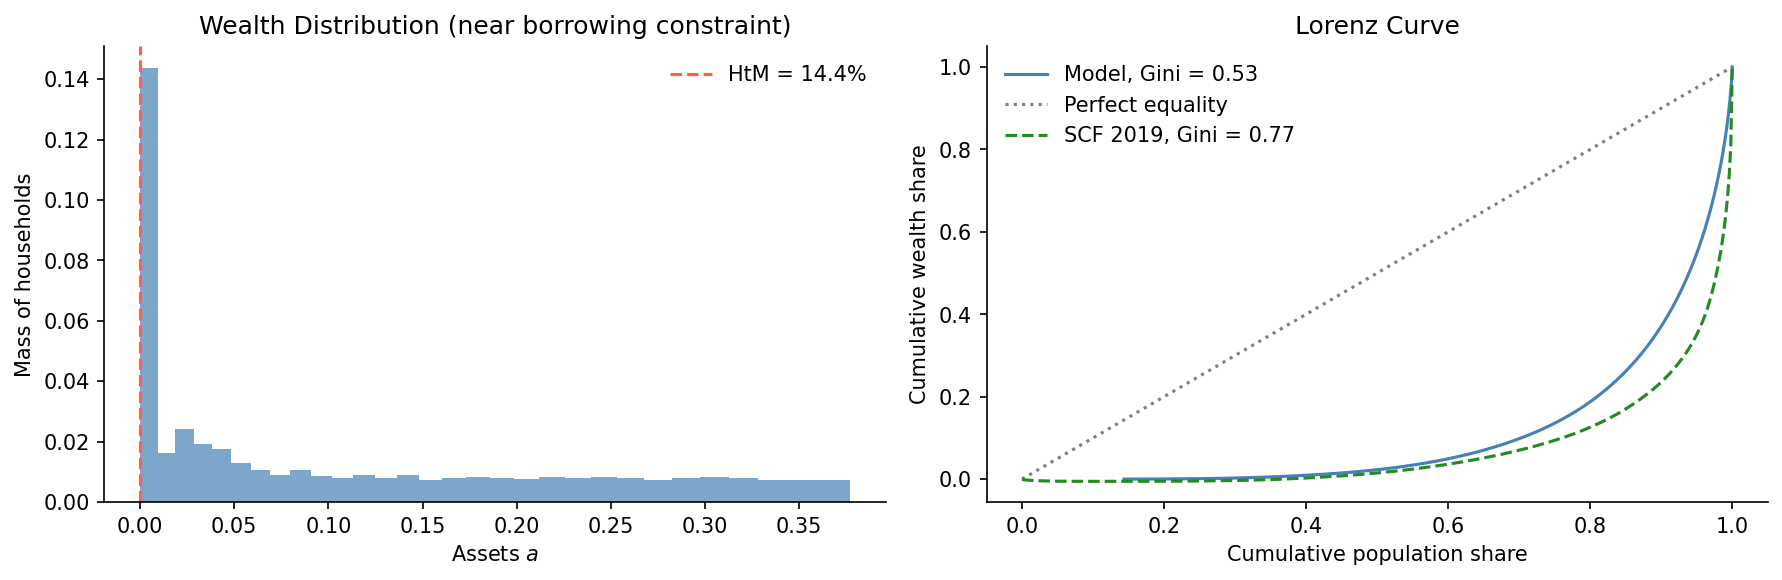
\includegraphics[width=1\linewidth]{wealth_distribution.png}
    \caption{Wealth Distribution}
    \label{fig:wealth_distribution}
\end{figure}


%---------------------------------------------------
% Descriptive Statistics
%---------------------------------------------------
\begin{table}[htbp]
\centering
\caption{Steady State: Bolsa Fam\'ilia vs.\ No-Transfer Counterfactual}
\label{tab:bf_ss}
\small
\begin{tabular}{lccc}
\toprule
 & With BF & No BF & $\Delta$ \\
\midrule
Formal Share $\alpha_F$ & 49.8\% & 49.9\% & -0.1 \\
Informal Share $\alpha_I$ & 44.5\% & 44.0\% & +0.5 \\
Unemployment $\alpha_U$ & 5.6\% & 6.0\% & -0.4 \\
Hand-to-Mouth & 13.9\% & 9.6\% & +4.3 \\
Wealth Gini & 0.802 & 0.783 & +0.019 \\
Consumption Gini & 0.443 & 0.452 & -0.009 \\
Aggregate Consumption $C$ & 1.336 & 1.340 & -0.004 \\
BF Spending & 0.027 & 0.000 & +0.027 \\
Welfare $\mathbb{E}[V]$ & -19.534 & -20.813 & +1.279 \\
\bottomrule
\end{tabular}
\end{table}
%---------------------------------------------------



\begin{figure}[H]
    \centering
    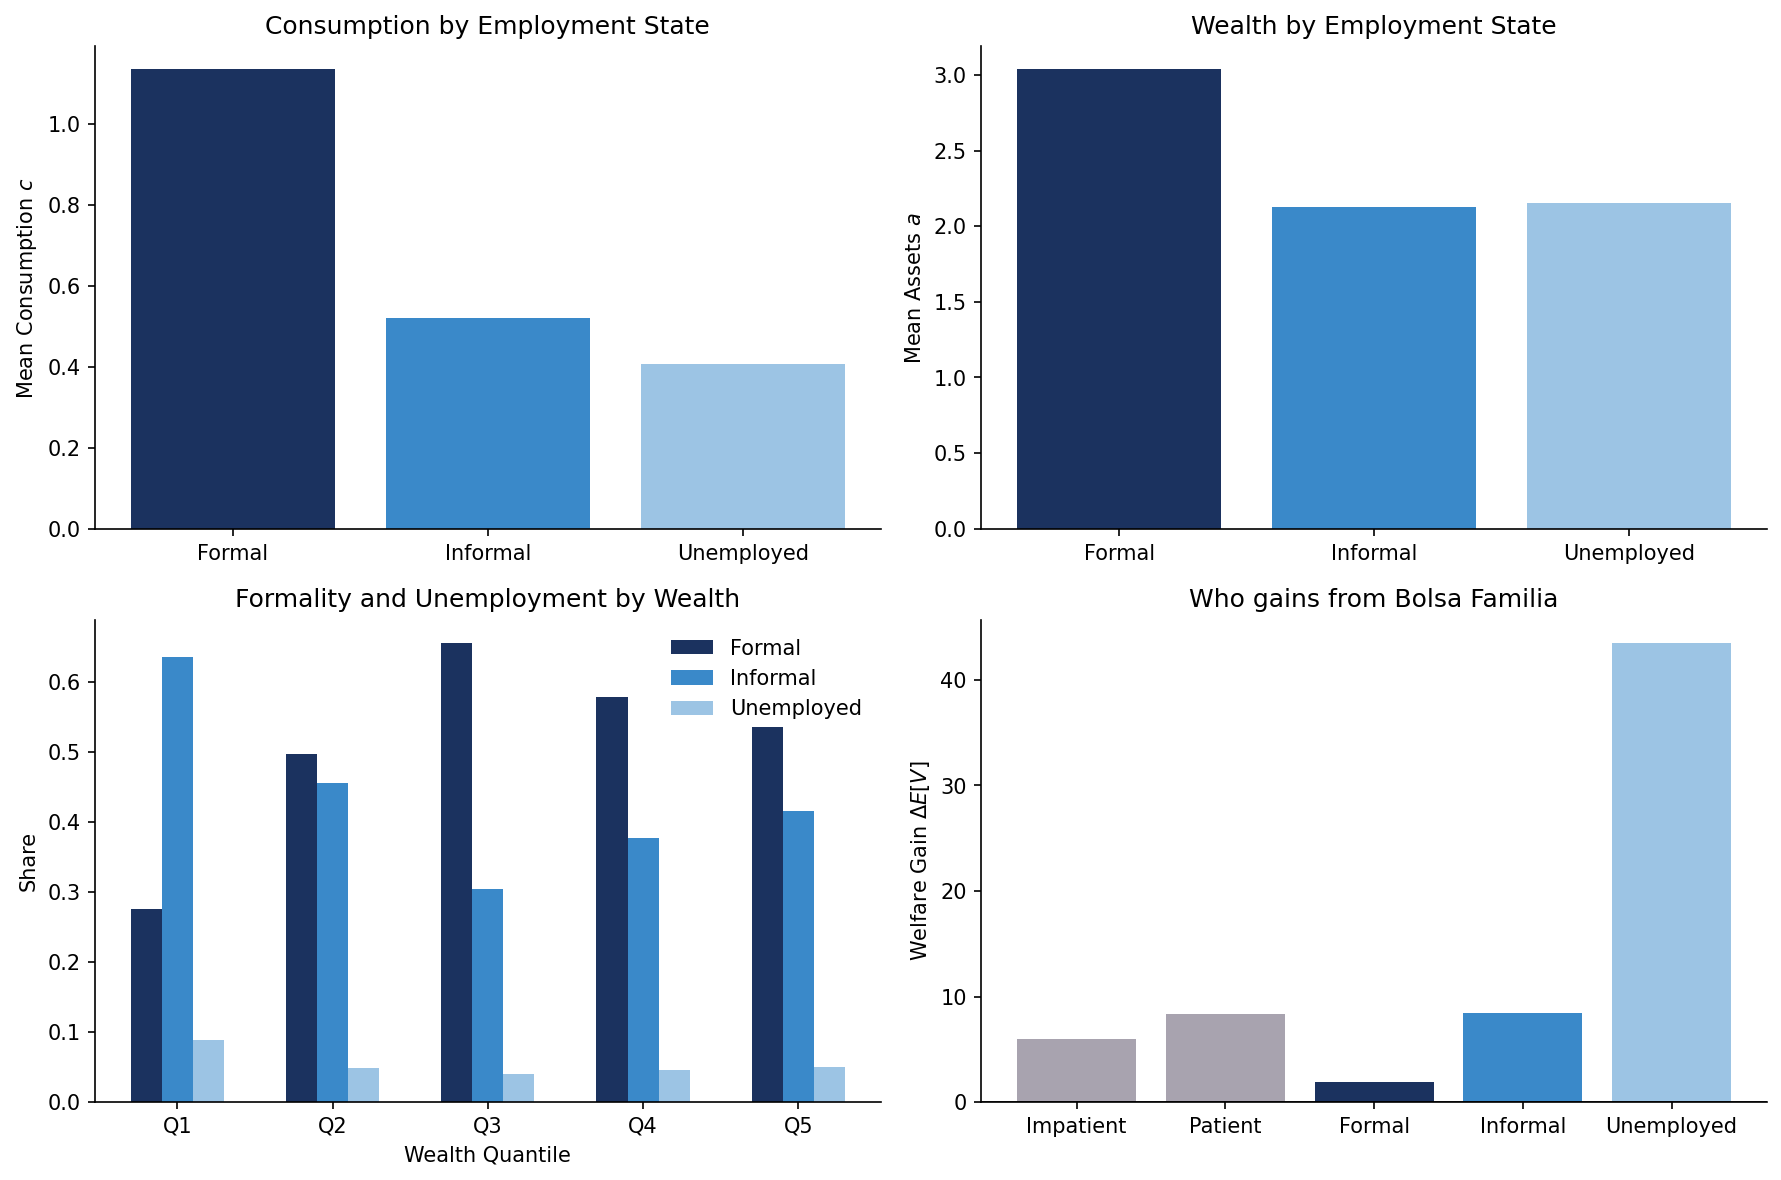
\includegraphics[width=1.0\linewidth]{bf_descript.png}
    \caption{Steady-State Descriptive Statistics}
    \label{fig:bf_descript}
\end{figure}


\begin{figure}[H]
    \centering
    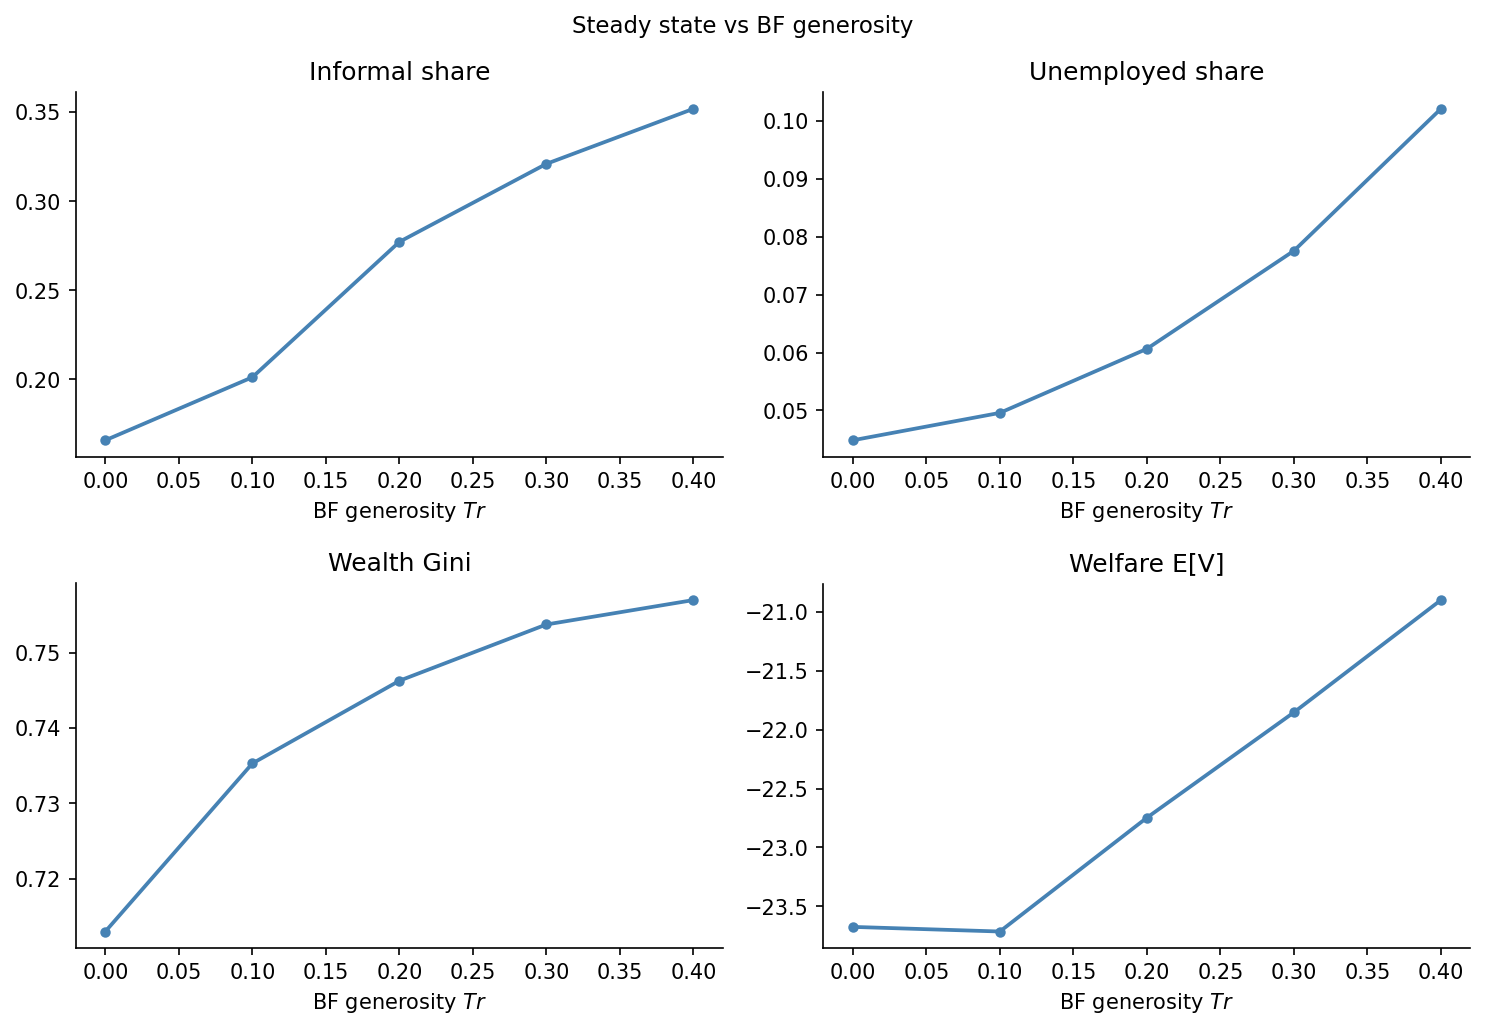
\includegraphics[width=1.0\linewidth]{bf_sweep.png}
    \caption{Steady-State Sensitivity Analysis}
    \label{fig:bf_sweep}
\end{figure}


%---------------------------------------------------
% Partial and General IRFs
\begin{figure}[H]
    \centering
    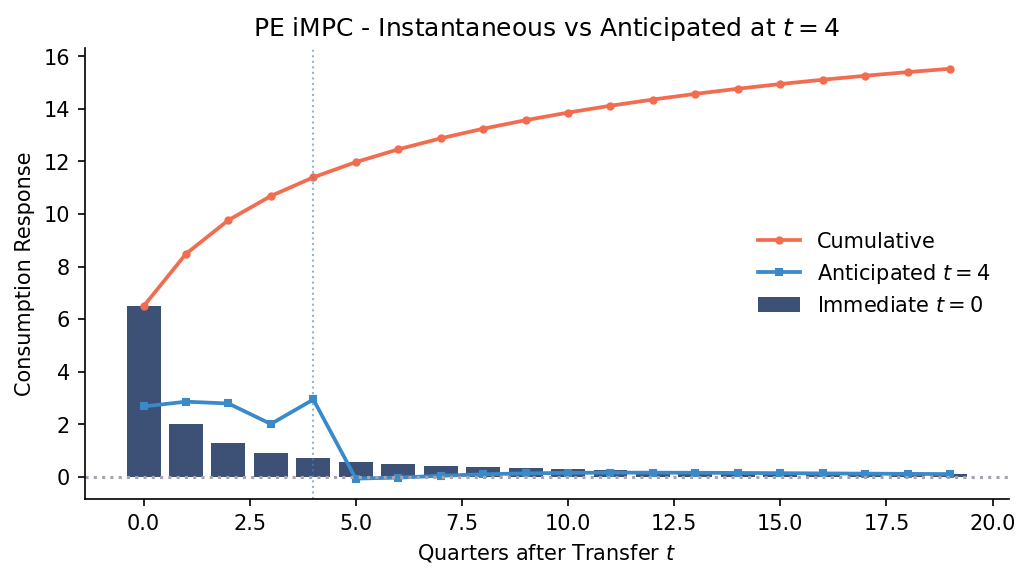
\includegraphics[width=0.9\linewidth]{impc.png}
    \caption{Partial Equilibrium iMPC}
    \label{fig:impc}
\end{figure}


\begin{figure}[H]
    \centering
    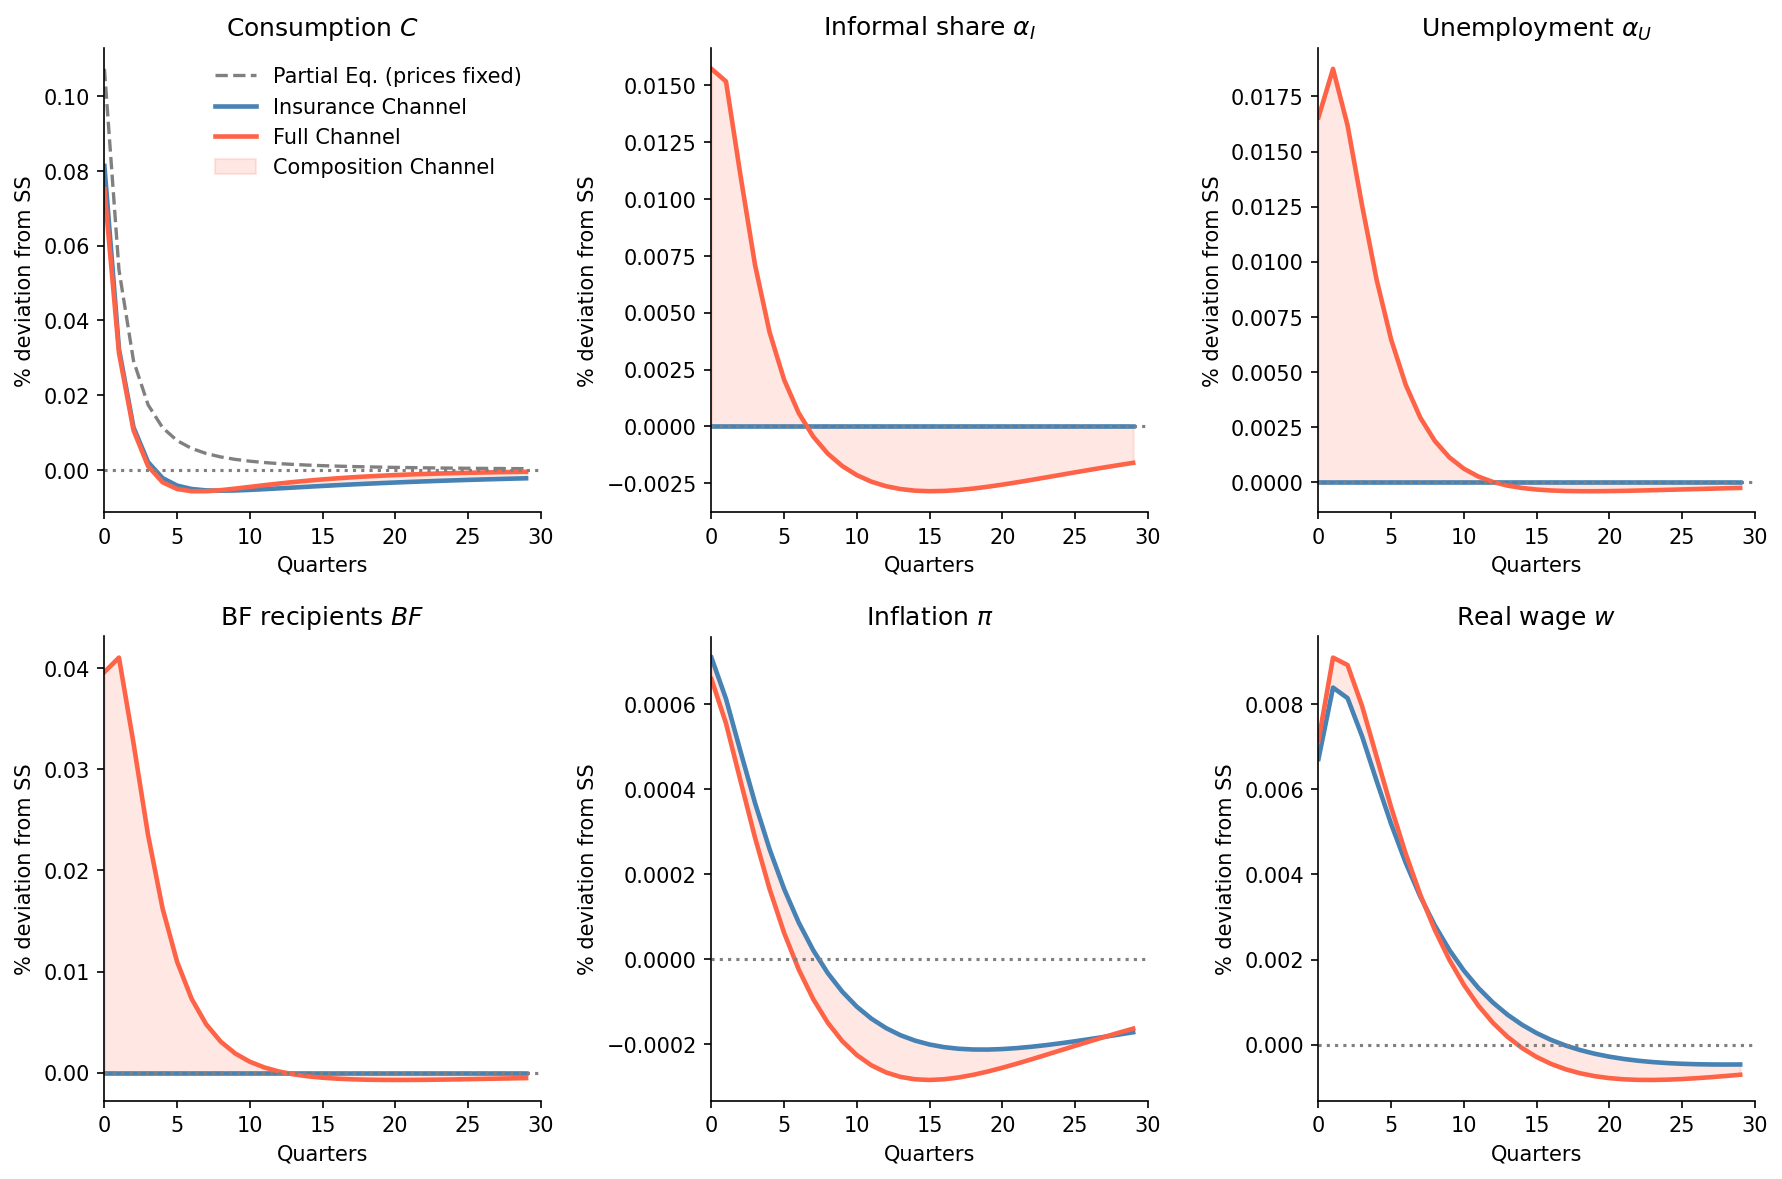
\includegraphics[width=1\linewidth]{irf_decomposition.png}
    \caption{IRFs: Insurance vs Composition Effect (shock in $T$)}
    \label{fig:irf_decomposition}
\end{figure}


\begin{figure}[H]
    \centering
    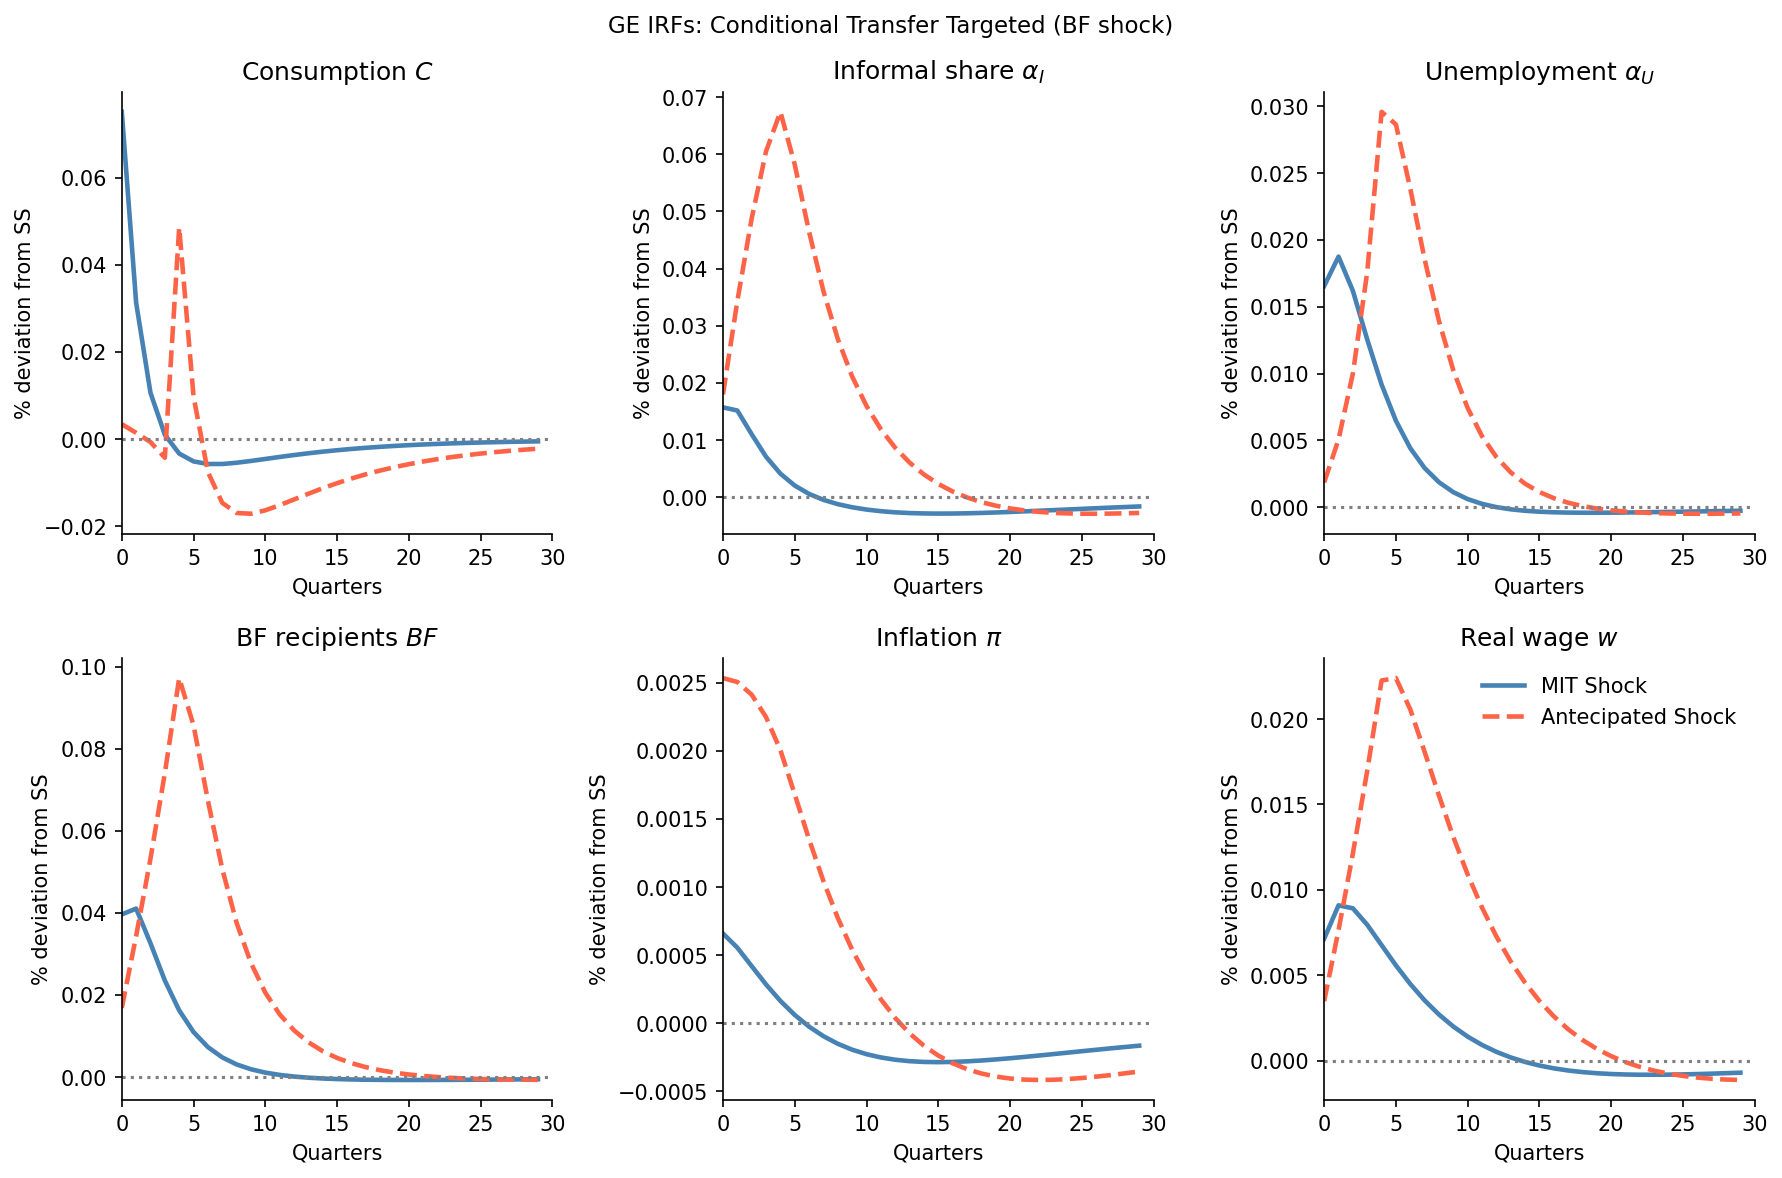
\includegraphics[width=1\linewidth]{irf_antecipated.png}
    \caption{IRFs: MIT vs Antecipated Shock (shock in $T$)}
    \label{fig:irf_antecipated}
\end{figure}

\begin{table}[htbp]\centering
\caption{Response in Consumption: Different Horizons}
\label{tab:response_consump}
\begin{tabular}{ccccc}
\toprule
 Horizon & Insurance & Full & Composition & Comp.\ (\%) \\\midrule
 4 & 0.0013 & 0.0012 & -0.0001 & -7.8 \\
 8 & 0.0011 & 0.0010 & -0.0001 & -12.2 \\
 20 & 0.0005 & 0.0006 & 0.0000 & 7.4 \\
 100 & -0.0003 & 0.0004 & 0.0007 & 158.2 \\
\bottomrule
\end{tabular}
\end{table}



%---------------------------------------------------
%	ROBUSTNESS TESTS
%---------------------------------------------------
\subsubsection*{Robustness Tests}

Lastly, in order to verify whether this results are representatives and robust,
we intent to do some robustness tests changing some calibration parameters,
such as $\gamma$, $\delta_\beta$, $\omega_I$, $\xi$, $\mu$, and $\kappa_w$.
This parameters might have minor implications in the results, but it is expected
that the model continues to have the same results.

Also, we intent to perform other dividend specifications instead of
$d_{i,t} = d_t \cdot e_{i,t}$. We also aim to change the GHH utility
to a standard separable utility in the form of $u(c) - v(h)$, which must have
similar results.


%---------------------------------------------------
%	BIBLIOGRAPHY
%---------------------------------------------------

\newpage

\singlespace

\printbibliography

%---------------------------------------------------
%	APPENDIX
%---------------------------------------------------

\newpage

\section*{Appendix}

% which means that the marginal value of the assets $V_a$ is
% \[
% V_a = \frac{\partial V_{t+1}}{\partial a'}
% = \frac{\partial V}{\partial c} \cdot \frac{\partial c}{\partial a}
% = (1+r_{t+1}) c^{-\frac{1}{\gamma}},
% \]

% and the Envelope Condition tells us that
% \[
% u'(c_t) = c_t^{-\frac{1}{\gamma}} = \beta \E_t [V_a^{t+1}]
% = \beta \E_t \left[ (1+r_{t+1}) c_{t+1}^{-\frac{1}{\gamma}} \right].
% \]

% Thus, we can create an inverse backwards iteration function of $V_a^{t}$ with
% respect to $V_a^{t+1}$, which is the central idea of the EGM.

\subsubsection*{Price Phillips Curve}

Let $Y_t$ be the aggregate output of the economy, a CES of the intermediary inputs,
\[
Y_t = \left(
    \int_0^1 y_{j,t}^\frac{\varepsilon-1}{\varepsilon} \: dj 
\right)^\frac{\varepsilon}{\varepsilon-1}.
\]

This firm maximizes its output subject to $\int_0^1 p_{i,j} y_{i,j} \; dj$.
The FOC implies that the demand for the intermediate good is given by
\[
y_{j,t} = \left( \frac{p_{j,t}}{P_t} \right)^{-\varepsilon} Y_t,
\]
where $P_t$ is the equilibrium price of the final good,
\[
P_t = \left( \int_0^1 p_{j,t}^{1-\varepsilon} \; dj \right)^{\frac{1}{1-\varepsilon}}.
\]

We assume a \textcite{rotemberg1982monopolistic} quadratic price
adjustment cost given by
\[
\frac{\theta_p}{2} \left( \frac{p_{j,t}}{p_{j,t-1}} - \bar \Pi \right)^2 Y_t,
\]
where $\theta_p = (\varepsilon-1) / \kappa$ is the adjustment cost multiplier
and $\bar \Pi$ the steady-state inflation.

Let $\Xi(y)$ be the intermediary firm's cost. Given last period's price $p_{j,t-1}$,
the firm chooses this period's price $p_{j,t}$ to maximize the present discounted
values of future profits,
\[
V_t^{IF}(p_{j,t-1}) = \max_{p_{j,t}} \frac{p_{j,t}}{P_t} y_{j,t} - \Xi(y_{j,t})
- \frac{\theta_p}{2} \left( \frac{p_{j,t}}{p_{j,t-1}} - \bar \Pi \right)^2 Y_t
+ \frac{1}{1+r_{t+1}} V_{t+1}^{IF} (p_{j,t}).
\]

We can replace the demand function into this problem, so
\[
V_t(p_{j,t-1}) = \max_{p_{j,t}} \frac{p_{j,t}}{P_t}
\left( \frac{p_{j,t}}{P_t} \right)^{-\varepsilon} Y_t - \Xi(y_{j,t})
- \frac{\theta_p}{2} \left( \frac{p_{j,t}}{p_{j,t-1}} - \bar \Pi \right)^2 Y_t
+ \frac{1}{1+r_{t+1}} V_{t+1} (p_{j,t}).
\]

The FOC with respect to $p_{j,t}$ is
\[
(1-\varepsilon) \left( \frac{p_{j,t}}{P_t} \right)^{-\varepsilon} \frac{Y_t}{P_t}
+ \varepsilon mc_{j,t} - \theta_p \left( \frac{p_{j,t}}{p_{j,t-1}} - \bar \Pi \right)
\frac{Y_t}{p_{j,t}} + \frac{1}{1+r_{t+1}} V'_{t+1}(p_{j,t}) = 0,
\]
where $mc_t = \partial \Xi / \partial y_{j,t}$, and the envelope condition gives us
\[
V_{t+1}' = \theta_p \left( \frac{p_{j,t+1}}{p_{j,t}} - \bar \Pi \right)
\frac{p_{j,t+1}}{p_{j,t}} \frac{Y_{t+1}}{p_{j,t}}.
\]

Thus, taking $p_{j,t} = P_t$ in equilibrium,
\[
\theta_p (\pi_t - \bar \Pi) \pi_t
= \varepsilon \left( mc_t - \frac{\varepsilon-1}{\varepsilon} \right)
+ \frac{1}{1+r_{t+1}} \theta_p (\pi_{t+1} - \bar \Pi) \pi_{t+1} \frac{Y_{t+1}}{Y_t},
\]
where we define the firm's markup as $\mu = \frac{\varepsilon}{\varepsilon-1}$.
Linearizing around the steady-state $\pi_t = \bar \Pi$,
\[
\ln (1+\pi_t)
= \frac{\varepsilon}{\theta_p} \left( mc_t - \frac{1}{\mu} \right)
+ \frac{1}{1+r_{t+1}}\ln (1+\pi_{t+1}) \frac{Y_{t+1}}{Y_t},
\]
where $\kappa = \varepsilon / \theta_p$ and $mc_t = w_t / Z_t$. This environment
is equivalent to \textcite{calvo1983staggered} in first order around zero inflation.

\subsubsection*{Wage Phillips Curve}

We will use the same setting as \textcite{hagedorn2019fiscal}, but considering just
the formal sector. Assume there is a union that aggregate effective labor input into
\[
h_t = \left(
    \int_0^1 e_{i,t} (h_{i,t})^\frac{\varepsilon_w-1}{\varepsilon_w} \: di 
\right)^\frac{\varepsilon_w}{\varepsilon_w-1},
\]
sells households labor services $e_{i,t} h_{i,t}$ at nominal wage $W_{i,t}$ to the
labor recruiter, which minimizes costs $\int_0^1 W_{i,t} e_{i,t} h_{i,t} \; di$,
implying a demand of
\[
h_{i,t} = \left( \frac{W_{i,t}}{W_t} \right)^{-\varepsilon_w} h_t.
\]

The unions sets a nominal wage $\hat W_t$ for an effect unit of labor,
$W_{i,t} = \hat W_t$ to maximize profits subject to
\textcite{rotemberg1982monopolistic}'s wage adjustment costs
\[
e_{i,t} \frac{\theta_w}{2}
\left( \frac{\hat W_{t}}{\hat W_{t-1}} - \bar \Pi^w \right)^2 h_t.
\]
We assume that the union's wage setting problem is
\[
V_t^w = \max_{\hat W_t} \int \left[
 \frac{(1-\tau_\ell)\hat W_t}{P_t} e_{i,t} h_{i,t}
- \frac{v(h_{i,t})}{u'(\tilde C_t)}
- e_{i,t} h_t \frac{\theta_w}{2}
\left( \frac{\hat W_t}{\hat W_{t-1}} - \bar \Pi^w \right)^2
\right] d\Lambda + \bar \beta V_{t+1}^w.
\]

Using the same algebra as the price Phillips curve, assuming that the union
allocates the same amount of hours in each worker $h_{i,t} = h_t$, and using
$\int_F e_{i,t} d\Lambda = L_t$, it is possible to find that
\[
\theta_w (\pi_t^w - \bar \Pi^w) \pi_t^w
= \varepsilon_w \left[ \frac{v'(h_t)}{u'(\tilde C_t)}
- \frac{\varepsilon_w-1}{\varepsilon_w} (1-\tau_\ell) w_t L_t \right]
+ \bar \beta \theta_w (\pi_{t+1}^w - \bar \Pi^w) \pi_{t+1}^w \frac{h_{t+1}}{h_t},
\]
which we can linearize around the steady state $\pi_t^w = \bar \Pi^w$ and take
$h_{t+1} = h_t$, since there is no population nor technological growth. Thus,
\[
\ln (1+\pi_t^w)
= \frac{\varepsilon_w}{\theta_w} \left[ \frac{v'(h_t)}{u'(\tilde C_t)}
- (1-\tau_\ell) w_t L_t \frac{\varepsilon_w-1}{\varepsilon_w} \right]
+ \bar \beta \ln (1+\pi_{t+1}^w).
\]

Therefore, defining $\kappa_w = \varepsilon_w/\theta_w$ and
$\mu_w = \varepsilon_w/(\varepsilon_w-1)$, the wage Phillips curve is
\[
\ln (1+\pi_t^w)
= \kappa_w \left[ \psi \cdot h_t^{1/\varphi} \cdot \tilde C_t^{1/\gamma}
- \frac{(1-\tau_\ell) w_t L_t}{\mu_w}  \right]
+ \bar \beta \ln (1+\pi_{t+1}^w).
\]



\end{document}
